\documentclass[../report.tex]{subfiles}
\begin{document}
\section{Phase 3}
Cette section documente le travail réalisé pour atteindre les fonctionnalités de la phase 3 du projet. En plus de fonctionnalités de la phase 2 (faits avec support des variables), on rajoute le support des clauses "complexes", c'est à dire avec un corps. On rajoute également le support des listes.
\subsection{Besoins}
Les besoins de cette phase sont les suivants :
\begin{itemize}
    \item Ajout du support des clauses complexes au parser, avec leur représentation en Java 
    \item Ajout du support des listes au parser, avec leur représentation en Java
    \item Implémentation de l'arbre de preuve pour résoudre les buts
\end{itemize}
\subsection{Plan}
Comme pour les phases précédentes, le plan va être de commencer par trouver une représentation Java pour les nouveaux éléments, puis adapter le parser pour ceux-ci. Enfin, on va adapter le noeud de résolution pour inclure l'arbre de preuve.
\subsection{Représentation des éléments}
Quelques ajouts et modifications sont nécessaires pour représenter correctement les nouveaux éléments. Ces changements sont décrits en détail dans les sections suivantes, et le diagramme de classe résultant est montré avec la figure \ref{fig:part3classdiagram}.
\subsubsection{Listes}
Une liste en Prolog n'est rien d'autre qu'une structure récursive avec le foncteur \texttt{'.'}, comme le montre la figure \ref{fig:phase3internallist}. On va donc profiter de cette représentation interne pour ne pas devoir dupliquer les opérations d'unification et autres. Ce qui se traduit en code par un héritage depuis de \mintinline{Java}{ProloGraalStructure}. En plus des sous-termes d'une structure classique, on va également garder directement une liste interne des éléments de la liste, ainsi qu'une référence directe vers la queue de la liste. Ces éléments ne sont pas directement utilisés à part au moment de la construction; cependant, ils pourraient servir à d'éventuelles optimisations\footnote{En l'état actuel, il n'est donc pas très utile de faire la différence entre les listes et les structures...}.
\begin{figure}[h]
    \centering
    \begin{tikzpicture}
        \Tree [.\texttt{'.'/2} v1 [.\texttt{'.'/2} v2 [.\texttt{'.'/2} v3 [.\texttt{[]} ] ] ] ]
        \end{tikzpicture}
    \caption{Représentation interne de la liste \mintinline{Prolog}{[v1,v2,v3]}}
    \label{fig:phase3internallist}
\end{figure}
La méthode clé de la représentation est celle permettant de créer la représentation interne de la liste. Elle va remplir les sous-termes de la structure avec les bon élément \texttt{'.'}. Comme les listes Prolog sont récursives par nature, l'implémentation l'est également. Le procédé est le suivant : on garde un lien vers la structure courante. On met son foncteur au foncteur \texttt{'.'}. Pour chaque élément de la liste jusqu'à l'avant-dernier, on l'ajoute comme premier sous-terme de la structure courante. On crée une nouvelle structure avec comme foncteur toujours \texttt{'.'}. Enfin, on ajoute cette nouvelle structure comme deuxième sous-terme de la structure courante, et la nouvelle structure devient la courante. Pour le dernier élément, on l'ajoute en temps que sous-terme de la structure courante, comme pour les précédents, mais le second sous-terme n'est plus une structure \texttt{'.'/2} mais la queue de la liste.
\begin{minted}[breaklines]{Java}
// list elements
protected List<ProloGraalTerm<?>> items;
// tail of the list. Empty by default, but a setter is provided.
protected ProloGraalTerm<?> tail = ProloGraalBuiltinAtoms.EMPTY_LIST;

/**
 * Create the parent structure based on the internal representation of a Prolog list. 
 */
public void buildInteralRepresentation() {
    this.setFunctor(ProloGraalBuiltinAtoms.DOT_OPERATOR);
    ProloGraalStructure struct = this;
    // for each item until the tail
    for(int i = 0; i < items.size()-1; i++) {
        ProloGraalTerm<?> item = items.get(i);
        // add "left side" to the representation
        struct.addSubterm(item);
        // create "right side" of the representation
        ProloGraalStructure next = new ProloGraalStructure(variables);
        next.setFunctor(ProloGraalBuiltinAtoms.DOT_OPERATOR);
        // add "right side"
        struct.addSubterm(next);
        // switch to the new structure on the right side
        struct = next;
    }
    ProloGraalTerm<?> item = items.get(items.size()-1);
    struct.addSubterm(item);
    struct.addSubterm(this.tail);
}
\end{minted}
\subsubsection{Clauses}
Une clause est composée d'une tête, qui est un terme, et une liste de buts, qui sont également des termes. La représentation d'une clause n'a pas vraiment d'intelligence, elle sert uniquement à stocker la tête et les buts.
\begin{figure}[h]
    \centering
    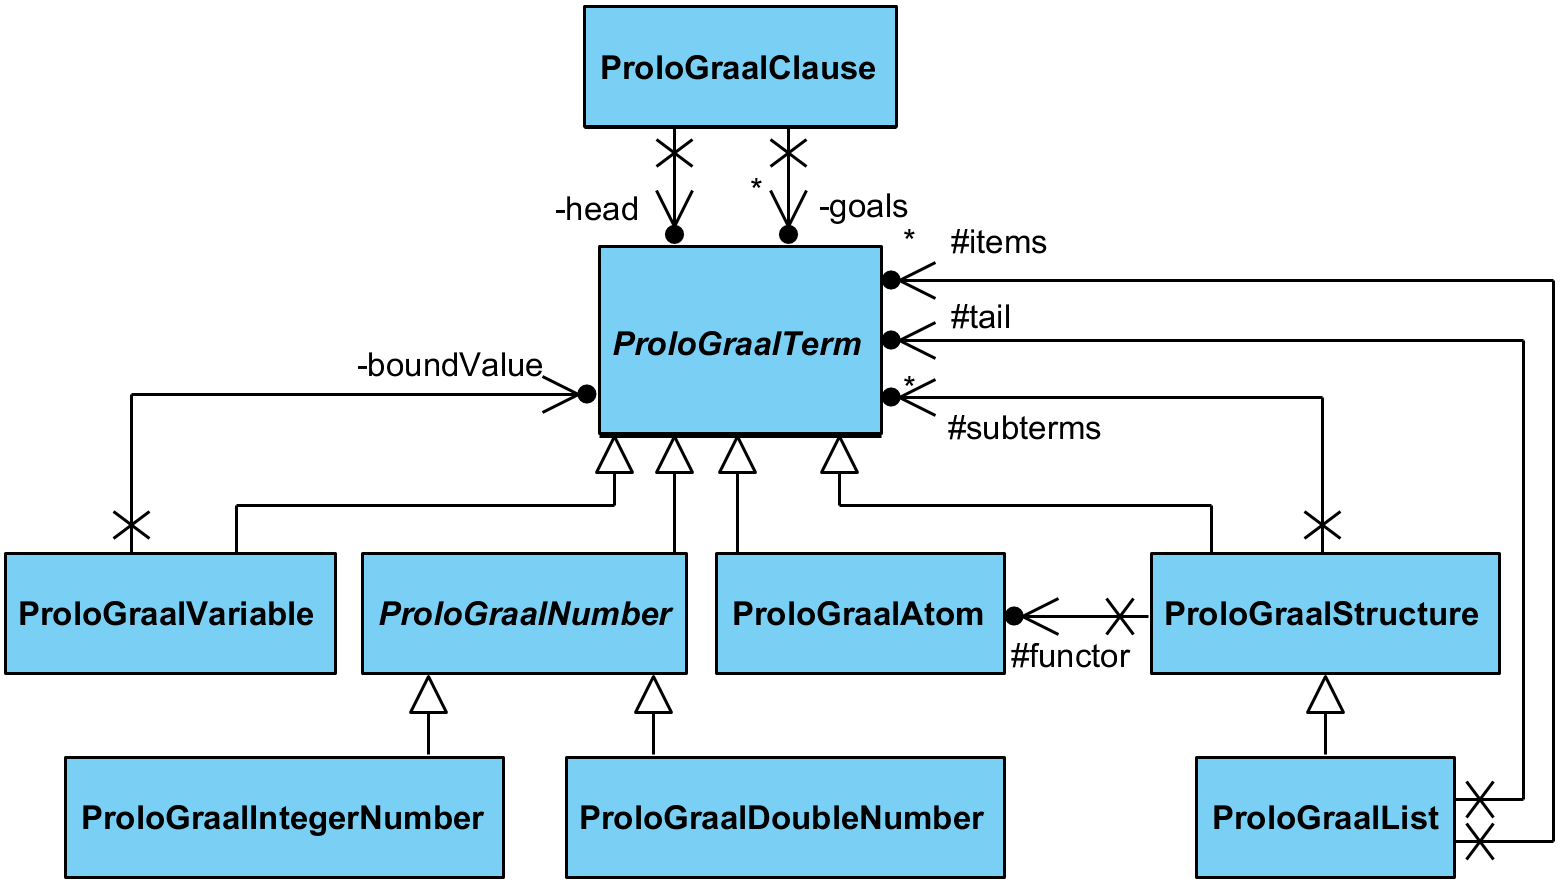
\includegraphics[width=\textwidth]{part3classdiagram.png}
    \caption{Diagramme de classes des éléments Prolog en Java, avec listes et clauses}
    \label{fig:part3classdiagram}
\end{figure}
\subsection{Adaptation du parser}
Les modifications suivantes sont à faire dans tout le trio lexer-parser-listener :
\begin{itemize}
    \item Ajouter les listes
    \item Ajouter les clauses complexes
\end{itemize}
\subsubsection{Lexer}
Dans le lexer, on doit rajouter les nouveaux éléments suivantes : les délimiteurs de liste \texttt{[} et \texttt{]}, le marqueur de queue de liste \texttt{|}, la virgule pour séparer les buts et les éléments des listes, et finalement le marqueur de corps de clause \texttt{:-} :
\begin{minted}{ANTLR}
LIST_START : '[';
LIST_END : ']';
LIST_ENDING : '|';    
SEPARATOR : ',';
CLAUSE_MARKER : ':-';
\end{minted}
\subsubsection{Parser}
Dans le parser, on doit maintenant utiliser nos nouveaux éléments de lexer. On commence par la liste vide, qui est un atome :
\begin{minted}{ANTLR}
atom :
ATOM |
LIST_START LIST_END // empty list
;    
\end{minted}
Puis on définit la liste, qui commence par un \texttt{[} et se termine par un \texttt{]}, qui contient un ou plus termes séparés par une virgule, et qui se termine optionnellement par un \texttt{|} suivi d'une queue. La queue est un terme quelconque.
\begin{minted}{ANTLR}
tail :
term
;

list :
LIST_START
term (SEPARATOR term)* (LIST_ENDING tail)?
LIST_END
;
\end{minted}
On continue en modifiant le terme pour inclure la possibilité qu'il soit une liste. On extrait également la définition du terme composé, qui était auparavant incluse dans la définition du terme, pour pouvoir la réutiliser indépendamment plus tard :
\begin{minted}{ANTLR}
composedTerm :
functor ('(' term (',' term)* ')') 
;

term :
composedTerm |
atom | 
number |
variable | 
list
;
\end{minted}
On définit ensuite la clause, qui peut être soit un fait, soit une clause composée (ou clause complexe).
\begin{minted}{ANTLR}
clause :
fact |
composedClause
;    
\end{minted}
Une clause composée est constituée d'une tête, qui peut être un atome ou un terme composé, suivie du marqueur de corps \texttt{:-}, suivi d'un certain nombre de buts séparés par des virgules qui peuvent chacun être un atome ou un terme composé. Enfin, la clause se termine par un point.
\begin{minted}{ANTLR}
head :
atom |
composedTerm
;

goal :
atom |
composedTerm
;

composedClause :
head CLAUSE_MARKER goal (SEPARATOR goal)* TERMINATOR
;
\end{minted}
Même si la tête et les buts peuvent être composés par les mêmes éléments, la distinction est quand même faite pour faciliter le travail du listener.
\subsubsection{Listener}\label{subsubsec:phase3listener}
Le listener a été complètement repensé pour cette étape, avec une manière de faire bien plus simple qu'avant. Au lieu des différentes listes (cf. \ref{subsubsec:listenerImpl}), on utilise deux piles : une pour les éléments divers que l'on rencontre au fur et à mesure, et une autre pour les clauses.
\begin{minted}{Java}
private Deque<ProloGraalTerm<?>> elements = new ArrayDeque<>();
private Deque<ProloGraalClause> clauses = new ArrayDeque<>();
\end{minted}
On utilise la classe \mintinline{Java}{ArrayDeque} plutôt que la classe \mintinline{Java}{Stack} pour les raisons suivantes, tirées de la documentation officielle :
\begin{itemize}
    \item Stack : \textit{A more complete and consistent set of LIFO stack operations is provided by the Deque interface and its implementations, which should be used in preference to this class.}\footnote{\href{https://docs.oracle.com/javase/8/docs/api/java/util/Stack.html}{https://docs.oracle.com/javase/8/docs/api/java/util/Stack.html}}
    \item ArrayDeque : \textit{This class is likely to be faster than Stack when used as a stack, and faster than LinkedList when used as a queue.}\footnote{\href{https://docs.oracle.com/javase/8/docs/api/java/util/ArrayDeque.html}{https://docs.oracle.com/javase/8/docs/api/java/util/ArrayDeque.html}}
\end{itemize}
On va ensuite profiter des événements d'entrée mais surtout de ceux de sortie pour ajouter les éléments aux bons endroits. Le principe est le suivant : quand on arrive à un élément "primitif", on en crée la représentation Java et on l'ajoute à la pile des éléments, sans se soucier de l'ajouter à une structure ou autre :
\begin{minted}[breaklines]{Java}
@Override
public void enterAtom(ProloGraalParser.AtomContext ctx) {
    ProloGraalAtom atom = new ProloGraalAtom(clauses.peek().getVariables(), ctx.getText());
    elements.push(atom);
}

@Override
public void enterList(ProloGraalParser.ListContext ctx) {
    elements.push(new ProloGraalList(clauses.peek().getVariables()));
}

@Override
public void enterComposedTerm(ProloGraalParser.ComposedTermContext ctx) {
    elements.push(new ProloGraalStructure(clauses.peek().getVariables()));
}
\end{minted}
De manière analogue, quand on entre dans une clause, on en crée une nouvelle et on l'ajoute à la pile des clauses :
\begin{minted}{Java}
@Override
public void enterClause(ProloGraalParser.ClauseContext ctx) {
    clauses.push(new ProloGraalClause());
}
\end{minted}
La logique s'effectue ensuite au moment de la sortie des éléments. Par exemple, quand on quitte un terme composé, on va enlever des éléments de la pile et les stocker dans une liste jusqu'à ce qu'on arrive à un élément de type "terme composé" encore vide. Cela signifie que l'on a atteint l'élément qui devra contenir les sous-termes accumulés dans la liste (en sens inverse, vu que les éléments arrivent d'une pile).
\begin{minted}{Java}
@Override
public void exitComposedTerm(ProloGraalParser.ComposedTermContext ctx) {
    List<ProloGraalTerm<?>> subterms = new ArrayList<>();
    while(true){
        while(!(elements.peek() instanceof ProloGraalStructure)) {
            subterms.add(elements.pop());
        }
        // check if element is a composed term already handled
        if(((ProloGraalStructure)elements.peek()).getArity() > 0) {
            subterms.add(elements.pop());
        } else {
            break;
        }
    }

    ProloGraalStructure struct = (ProloGraalStructure) elements.peek();
    for(int i = subterms.size()-1; i >= 0; i--) {
        struct.addSubterm(subterms.get(i));
    }
}
\end{minted}
Cette logique est très simple à utiliser pour les autres éléments également. Par exemple, quand on sort d'un foncteur, on sait que l'élément précédent était forcément la structure qui doit avoir ce foncteur :
\begin{minted}{Java}
@Override
public void exitFunctor(ProloGraalParser.FunctorContext ctx) {
    try {
        ProloGraalAtom functor = (ProloGraalAtom) elements.pop();
        ProloGraalStructure struct = (ProloGraalStructure) elements.peek();
        struct.setFunctor(functor);
    } catch(ClassCastException ex) {
        throwParseError(ctx, "Invalid state : " + ex.getLocalizedMessage());
    }
}
\end{minted}
Pour les variables, on reprend toujours le même concept de vérifier si la variable existe déjà avant de l'ajouter, mais pour assurer le fonctionnement il faut ajouter de toute façon la variable à la pile des éléments. 

On remarque qu'on l'ajoute également à la liste des variables de la clause. Cette liste correspond à celle qui était présente de manière globale dans les versions précédentes. Ce n'est cependant plus une liste, mais un dictionnaire, pour rendre la vérification plus rapide (plus besoin de chercher dans toute la liste). En fait, logiquement il s'agit d'un ensemble, mais l'implémentation du \texttt{Set} de Java ne permet pas de récupérer une valeur, uniquement de tester si oui ou non elle est présente à l'intérieur. Pour pallier ce problème, une \mintinline{Java}{Map<Variable, Variable>} est donc utilisée.
\begin{minted}[breaklines]{Java}
@Override
public void enterVariable(ProloGraalParser.VariableContext ctx) {
    ProloGraalVariable variable = new ProloGraalVariable(clauses.peek().getVariables(), ctx.getText());
    if(clauses.peek().getVariables().containsKey(variable)) {
        // add a reference to the previously added one
        elements.push(clauses.peek().getVariables().get(variable)); 
    } else {
        elements.push(variable);
        clauses.peek().getVariables().put(variable, variable);
    }
}
\end{minted}
Il faut encore gérer les listes. Une astuce est de retenir la queue de la liste au moment où l'on en sort. Cette astuce marche même dans le cas récursif où la queue serait également une liste, vu que l'on sortira d'abord de la liste interne, puis on passera dans \texttt{exitTail} ce qui mettra la queue pour la liste externe.
\begin{minted}{Java}
@Override 
public void exitTail(ProloGraalParser.TailContext ctx) {
    tail = elements.pop();
}
\end{minted}
Le code pour créer la liste est en suite très similaire à celui pour les structures, avec en plus la gestion de la queue et la création de la représentation interne :
\begin{minted}{Java}
public void exitList(ProloGraalParser.ListContext ctx) {
    // ...
    if(tail != null) {
        list.setTail(tail);
        tail = null;
    }
    list.buildInteralRepresentation();
}
\end{minted}
\subsubsection{Retour du parser}
Pour le retour du parser de la phase 2 (cf. \ref{subsubsec:phase2parser}), nous avions introduit la classe \mintinline{Java}{ProloGraalParseResult} pour stocker la liste des faits ainsi que les variables. Cette classe est renommée en \mintinline{Java}{ProloGraalRuntime}, et ne contient plus que les clauses du programme, les variables étant déjà inclues dans ces dernières. Mais ces clauses ne sont pas stockées dans une simple liste. On utilise un dictionnaire reliant une tête à une liste de clauses. Ceci permet de retrouver efficacement les clauses compatibles avec un certain but dans le noeud de résolution. Cette implémentation nécessite cependant l'effort supplémentaire de fournir une méthode \texttt{hashCode} fonctionnelle pour chacun des types de terme.
\begin{minted}{Java}
private final Map<ProloGraalTerm<?>, List<ProloGraalClause>> clauses;

public ProloGraalRuntime(List<ProloGraalClause> clauseList) {
    clauses = new HashMap<>();

    for (ProloGraalClause clause : clauseList) {
        clauses.putIfAbsent(clause.getHead(), new ArrayList<>());
        List<ProloGraalClause> clauses1 = clauses.get(clause.getHead());
        clauses1.add(clause);
    }
}
\end{minted}
Comme pour le \mintinline{Java}{ProloGraalParseResult}, ce résultat de parser est stocké dans le contexte et accessible depuis le noeud de résolution.
\subsection{Arbre de preuve}
Pour l'implémentation de l'arbre de preuve, plusieurs méthodes sont possibles. Les deux ayant été considérées sont les suivantes :
\begin{itemize}
    \item Méthode récursive utilisant la pile d'appels comme mécanisme pour le parcours de l'arbre
    \item Méthode utilisant une boucle pour simuler le parcours de l'arbre
\end{itemize}
La méthode récursive est plus facile à implémenter, mais est rapidement soumise aux limitations de taille de la pile d'appels. Malgré ce désavantage, c'est quand même cette version qui est retenue.

Le fonctionnement de l'arbre de preuve est le suivant : on maintient une liste de buts. On va ensuite remplacer le premier but par un corps possible (dont la tête s'unifie), ce qui crée un noeud par remplacement possible. On va ensuite recommencer cette opération jusqu'à ce qu'on atteigne des faits, ce qui aura pour effet de diminuer la taille de la liste des buts. On continue de recommencer le processus jusqu'à ce que la liste de buts soit vide, ce qui correspond à un succès, ou jusqu'à ce qu'on ne puisse plus remplacer, ce qui correspond à un échec.
\subsubsection{Noeud de résolution}
Le noeud de résolution sert maintenant à initialiser l'arbre de preuve. Il crée la liste de buts et donne le premier but, qui est la requête qui arrive depuis l'interpréteur. Il va ensuite démarrer le processus de résolution en créant et en exécutant un \texttt{ProloGraalProofTreeNode}.
\begin{minted}[breaklines]{Java}
ProloGraalTerm<?> head = goalRuntime.getFirstClause().getHead();

Deque<ProloGraalTerm<?>> goals = new ArrayDeque<>();
goals.push(head);
ProloGraalProofTreeNode proofTreeNode = new ProloGraalProofTreeNode(clauses, goals);

ProloGraalBoolean r = treeNode.execute();
\end{minted}
Un \texttt{Deque} est utilisé plutôt qu'une simple liste pour les buts, car les buts sont insérés au début (on pourrait aussi utiliser un \texttt{Stack} ou une \texttt{Queue}, mais les raisons citées à la section \ref{subsubsec:phase3listener} s'appliquent également ici).
\subsubsection{Noeuds de l'arbre de preuve}
Les noeuds de l'arbre de preuve sont responsables de remplacer le premier but par ses possibles corps, et de relancer le traitement récursivement. On commence donc par vérifier si la liste de buts est vide : cela signifie que nous avons atteint un succès, il faut donc le signaler en retournant un \texttt{ProloGraalSuccess}.
\begin{minted}{Java}
if(goals.isEmpty()) { // leaf node
    return new ProloGraalSuccess();
}
\end{minted}
On va ensuite récupérer le but actuel (le premier de la liste) ainsi que les candidats potentiellement unifiables. S'il n'y en a pas, alors on lève une erreur.
\begin{minted}{Java}
ProloGraalTerm<?> currentGoal = goals.getFirst();
List<ProloGraalClause> possibleClauses = clauses.get(currentGoal);
// if no match, throw an error
if(possibleClauses == null || possibleClauses.isEmpty())
    throw new ProloGraalExistenceError();
\end{minted}
On va ensuite essayer chacun de ces candidats, en essayant de les unifier avec le but courant. Mais on doit d'abord créer une copie du candidat, pour s'assurer de ne pas corrompre la base de clauses au moment de l'unification. On sauvegarde également l'état du but courant pour les mêmes raisons. 
\begin{minted}{Java}
for(ProloGraalClause possibleClauseOriginal : possibleClauses) {
    ProloGraalClause possibleClause = possibleClauseOriginal.copy();

    currentGoal.save();

    // if the head of the clause is unifiable with the current goal
    if(possibleClause.getHead().unify(currentGoal)) {
\end{minted}
Si l'unification ne fonctionne pas, alors il suffit de défaire tous les changements sur le but en appelant la méthode \texttt{undo}. Sinon, si l'unification a fonctionné, alors on va créer une nouvelle liste de buts et remplacer le premier par le corps du candidat :
\begin{minted}{Java}
// create a copy of the current goals
Deque<ProloGraalTerm<?>> newGoals = new ArrayDeque<>(goals);

List<ProloGraalTerm<?>> body = possibleClause.getGoals();

// always remove the first goal since it will be replaced
newGoals.pollFirst();

// no need for distinction between facts and regular clauses
Collections.reverse(body);
body.forEach(newGoals::addFirst);
\end{minted}
On remarque l'inversion des buts du corps du candidat. Elle est nécessaire vu que l'on ajoute les buts toujours au début de la liste.

Il ne reste plus qu'à créer et appeler un nouveau noeud en lui donnant la nouvelle liste de buts. À ce stade, on ne gère pas les résultats multiples, donc on retourne immédiatement si cet appel récursif donne un succès.
\begin{minted}{Java}
if(new ProloGraalProofTreeNode(clauses, newGoals).execute().asBoolean()) {
    return new ProloGraalSuccess();
}
\end{minted}
Finalement, il ne faut pas oublier que si l'on a essayé tous les candidats mais que tous ont échoué, alors il faut retourner un échec.
\subsubsection{Synthèse}
L'implémentation de l'arbre de preuve est maintenant terminée, en assumant un fonctionnement correct du mécanisme d'unification. Ce n'est cependant pas le cas, la phase précédente ayant laissé une unification très approximative. On va donc s'y repencher.
\subsection{Correction des problèmes d'unification}\label{subsec:unificationfixes}
Il y a principalement deux gros problèmes dans le mécanisme d'unification actuel des variables qui ont été omis :
\begin{itemize}
    \item Le concept de valeur racine
    \item Le test d'occurrence
\end{itemize}
\subsubsection{Valeur racine}
Quand on essaie d'unifier des variables, particulièrement entre-elles, il est important de toujours travailler sur la "valeur racine" de celles-ci. La valeur racine est le début de la possible chaîne de références d'une variable. Par exemple, si la variable \mintinline{Prolog}{A} est liée à \mintinline{Prolog}{B}, qui est elle même liée à la variable \mintinline{Prolog}{C}, qui est liée à l'atome \mintinline{Prolog}{x}, alors la valeur racine de \mintinline{Prolog}{A} doit être \mintinline{Prolog}{x}. L'implémentation précédente ne prenait pas en compte ce genre de cas, en ne regardant qu'à une distance maximum de 1. 

On implémente donc une méthode permettant de récupérer la valeur racine d'une variable, que l'on utilisera chaque fois que l'on a besoin de la valeur de cette variable. L'algorithme est simple : si la variable n'est pas liée, alors il s'agit de la racine. Sinon, on regarde à quoi est liée la variable. Si c'est une autre variable, alors on appelle cette méthode récursivement. Sinon, on retourne simplement la valeur liée.
\begin{minted}{Java}
@Override
public ProloGraalTerm<?> getRootValue() {
    if (this.isBound) {
        if (this.boundValue instanceof ProloGraalVariable) {
            return this.boundValue.getRootValue();
        } else {
            return this.boundValue;
        }
    } else {
        return this;
    }
}
\end{minted}
On utilise ensuite cette méthode lors de l'unification par exemple :
\begin{minted}{Java}
ProloGraalTerm<?> rootValue = other.getRootValue();
if (this.isBound) {
    return this.boundValue.getRootValue().unify(rootValue);
} else {
    this.bind(rootValue);
    return true;
}
\end{minted}
\subsubsection{Test d'occurrence}
Le test d'occurrence empêche l'unification d'une variable avec une structure la contenant. Par exemple, \mintinline{Prolog}{X} ne doit pas pouvoir s'unifier à \mintinline{Prolog}{f(X)}. L'implémentation de ce test est assez lourde, car on a besoin de maintenir la liste des variables présentes dans chaque structure, et on doit vérifier toutes les variables pour voir si leur valeur racine revient vers la variable que l'on cherche. On doit également vérifier récursivement si ces variables sont liés à d'autres structures :
\begin{minted}[breaklines]{Java}
private boolean occursCheck(ProloGraalStructure root) {
    Map<ProloGraalVariable, ProloGraalVariable> subVariables = root.getSubVariables();
    if (subVariables.get(this) == this) { // contains directly this
        return true;
    }
    for (ProloGraalVariable var : subVariables.values()) {
        ProloGraalTerm<?> rootValue = var.getRootValue();
        if (rootValue == this) { // or contains indirectly
            return true;
        }
        if (rootValue instanceof ProloGraalStructure) {
            if (occursCheck((ProloGraalStructure) rootValue)) {
                return true;
            }
        }
    }

    return false;
}
\end{minted}
On glisse ce test durant le processus d'unification :
\begin{minted}{Java}
ProloGraalTerm<?> rootValue = other.getRootValue();
if (rootValue instanceof ProloGraalStructure) {
    if (occursCheck((ProloGraalStructure) rootValue)) {
        return false;
    }
}
\end{minted}
\subsection{Affichage des résultats}
L'affichage des résultats est assez similaire à celui-ci de la phase 2. Le noeud de résolution encapsule les variables du but originel dans un succès :
\begin{minted}{Java}
if(r.asBoolean()) {
    r = new ProloGraalSuccess(head.getVariables());
}
return r;
\end{minted}
Et comme à la phase 2 ce succès est récupéré par l'interpréteur, et ses variables sont affichées.
\begin{minted}{Java}
if(callResult.asBoolean()) {
    ProloGraalSuccess success = (ProloGraalSuccess)callResult;
    for(ProloGraalVariable variable : success.getVariables().values()) {
        if(variable.isBound()) {
            ProloGraalTerm<?> root = variable.getRootValue();
            String rootStr;
            if(root instanceof ProloGraalStructure) {
                rootStr = ((ProloGraalStructure) root).toRootString();
            } else {
                rootStr = root.toString();
            }
            writer.println(variable.getName() + " = " + rootStr);
        }
    }
}
\end{minted}
Seule particularité, l'appel à une méthode \texttt{toRootString} dans le cas où une variable est liée à une structure. Cette méthode sert particulièrement dans le cas où la structure est une liste; elle va en effet formatter correctement la liste en la retransformant sous sa forme \texttt{[ ... ]}. Elle va également s'appliquer récursivement pour chaque variable contenue à l'intérieur de la structure, afin de produire un résultat correct pour l'affichage.
\subsection{Synthèse}
La phase 3 est maintenant terminée. Nous avons à présent un interpréteur fonctionnel, capable de résoudre des clauses complexes et de gérer des cas spéciaux de l'unification. Les objectifs initiaux du projet sont atteints. Les problèmes principaux restants sont les suivants :
\begin{itemize}
    \item Pas de gestion des requêtes multiples dans l'interpréteur.
    \item Impossible d'obtenir plus que le premier résultat.
\end{itemize}
\end{document}